\subsection{Financial News}
For extracting features describing the relationship among companies, financial news are chosen to be a good source of information. Most of the reviewed related work relies on news articles since its impact on the financial markets is a common presumption in the literature \cite{KhadjehNassirtoussi2014TextReview}. For this study, a dataset will be used consisting of financial news \footnote{https://drive.google.com/drive/folders/0B3C8GEFwm08QY3AySmE2Z1daaUE} released by \citet{Ding2014UsingInvestigation}. It contains news articles from Reuters \footnote{https://www.reuters.com} (106,519 documents) and Bloomberg \footnote{https://www.bloomberg.com} (448,395 documents) covering the time period from 2006-10-20 to 2013-11-26. Those texts will be used for extracting features like co-occurrences. How to extract these features and evaluate their informative value will be tackled in Section~\ref{section:text_analysis}.

Since this feature extraction will heavily rely on the content within articles, duplicated articles, empty articles and articles with a content length less than 300 characters will be removed.

\begin{figure}[!ht]
    \centering
    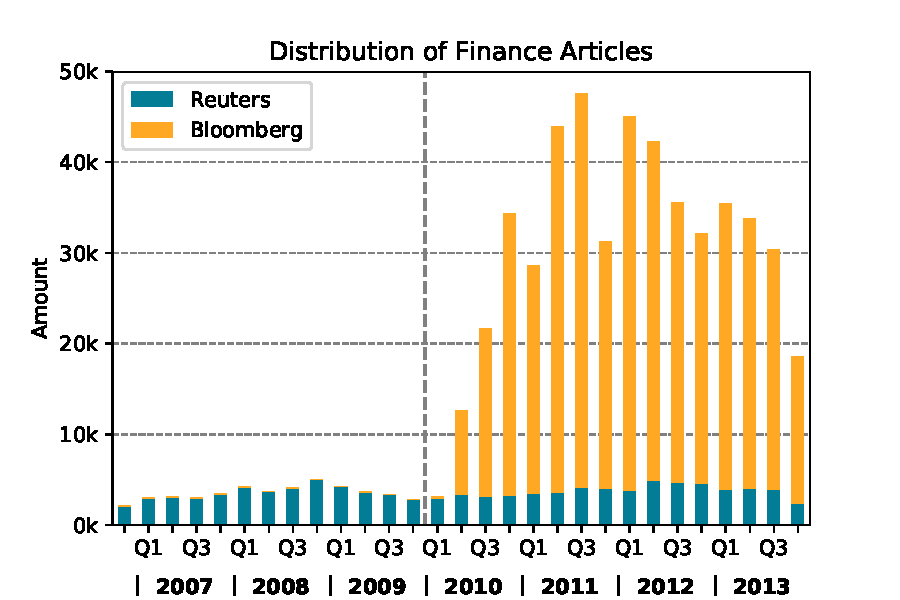
\includegraphics[width=0.8\textwidth]{figures/data/articles-distribution.pdf}
    \caption{Distribution in time for all articles after dropping empty, meaningless or duplicated ones. The dashed vertical line marks the beginning of the stock price dataset, introduced in the next step.}
    \label{fig:articles-distribution}
\end{figure}

After the most problematic properties of the data are tackled, there are 542,517 articles left. Figure~\ref{fig:articles-distribution} shows the distribution of these articles over time. While Reuters articles are equally distributed over all covered years, most of the Bloomberg articles are from 2010 until 2013.


\subsection{Stock Prices}
Stock prices are collected from a published dataset containing the historical prices for all components of the stock market index S\&P 500 from 2010 to the end 2016 \footnote{https://www.kaggle.com/dgawlik/nyse}. For each stock the daily open, high, low, close and volume values (OHLCV) are given in US dollar. The dataset already accounts for stock splits (Section~\ref{section:background}) by adjusting prices to the end of the time period. Thus, price values of affected stocks in 2010 are rectified to have the same meaning as in 2016.

For linking stock prices with occurrences in the previously introduced news dataset, we will be using the company names in the securities table from the same published dataset.

Since there are no financial news available after 2013-11-29, the stock prices after this week are discarded. However, the financial news before 2010 will be used, even though no stock prices are collected for this time period. The relational features which will be extracted are assumed to have a long-term impact, so it will be evaluated in Section~\ref{section:evaluation}, if incorporating information from news between 2006 and 2010 is helpful.

\begin{figure}[!ht]
    \centering
    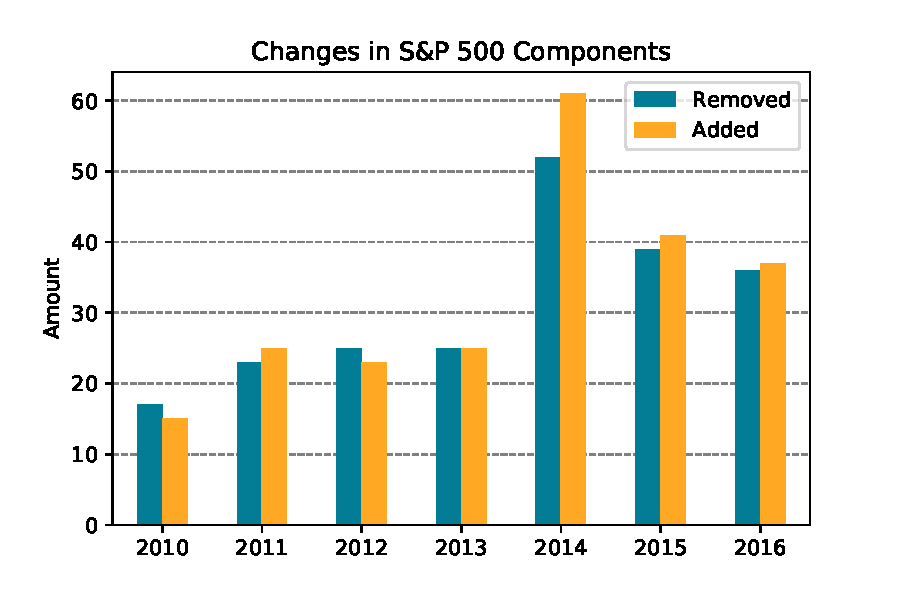
\includegraphics[width=0.8\textwidth]{figures/data/sp500-comp-changes.pdf}
    \caption{Starting with 499 components in 2010, the index underwent 217 removals and 227 additions until the end of 2016. The historical components for the S\&P 500 index were collected from an anonymous distribution page. \protect\footnotemark}
    \label{fig:sp500_changes}
\end{figure}

\footnotetext{https://nemozny.github.io/datasets/}

The selected stock price dataset accounts only for companies present in the S\&P 500 index at the end of 2016. As shown in Figure~\ref{fig:sp500_changes}, the index' components are continuously changing due to various reasons like acquisition, merger, dual-class listing or bankruptcy. Because we only have the prices for components from 2016, we ignore that some companies we are looking at are not actually part of the index during the observed time period. To avoid incomplete time series, stocks which were not continuously present are left out. In addition to the stock prices, overall measurements of the performance and the confidence at the NYSE for the same period as the stock prices need to be considered. Being popular variables for this purpose, the CBOE Volatility Index (VIX) \footnote{https://www.kaggle.com/lp187q/vix-index-until-jan-202018} and the S\&P 500 index (GSPC) \footnote{https://www.kaggle.com/benjibb/sp500-since-1950} are selected. As already observed by \citet{Fleming1995PredictingMeasure} when the VIX was introduced, there appears to be a strong negative relationship between volatility and stock market returns. Indicators supporting this assumption, can be seen in Figure~\ref{fig:index_and_vix} showing the closing values for both variables over the observed period. The first bursts of the VIX in 2010 and 2011 are hypothesized to be caused by important steps during the European debt crisis \footnote{https://money.cnn.com/2011/08/08/markets/vix\_fear\_index/index.htm}. The third burst is assumed to be a consequence of the \emph{1000-point plunge} of the DOW Jones index on the 24th of August in 2015 which in turn was a consequence of a rout in the Chinese market pulling down stock markets all over the world \footnote{https://money.cnn.com/2015/08/24/investing/stocks-markets-selloff-china-crash-dow/index.html}.

\begin{figure}[!ht]
    \centering
    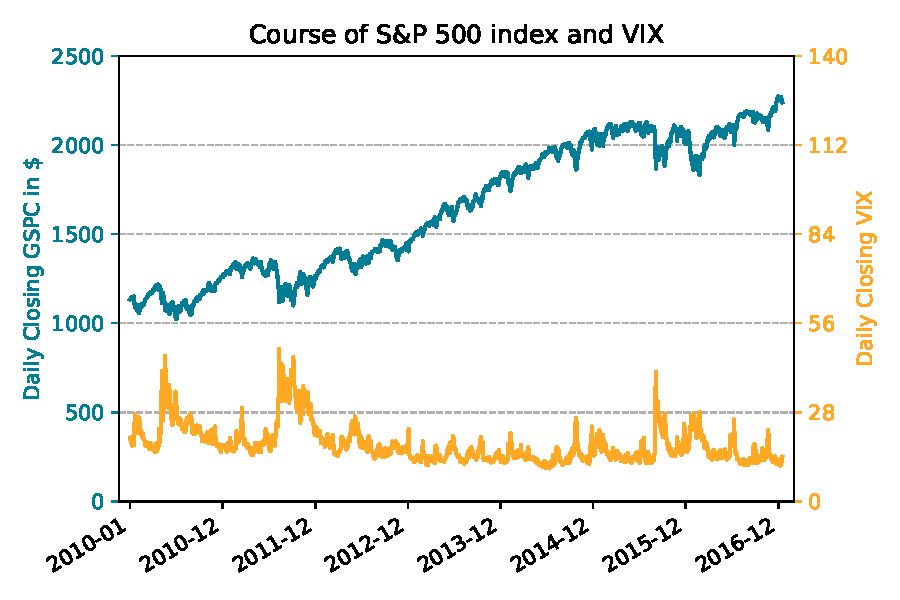
\includegraphics[width=0.8\textwidth]{figures/data/index-and-vix.pdf}
    \caption{Evolution of GSPC and VIX for the observed period. The scales are adjusted to visualize both time series close to each other in the same plot.}
    \label{fig:index_and_vix}
\end{figure}

The preselection ensures the complete stock prices of 467 companies for all 985 trading days from 2010-01-04 to 2013-11-29. % For evaluating prediction models all samples for the 189 trading days from 2013-03-01 on will be excluded during analysis and only used for final testing. The left over 794 trading days are used for the following analysis in Section~\ref{section:regression_analysis}.



% TODO: State: Only active trading days (holidays & weekends are excluded)


% Archived: Additionally it includes fundamental data extracted from Nasdaq Financials and SEC 10k annual fillings between 2012 and 2016. For each security essential information like ticker symbol, security name, address of headquarter, industry and sub industry are given.